\documentclass[10pt,conference,a4paper]{IEEEtran}

%import packages here
\usepackage{amsmath}
\everymath{\displaystyle}
\usepackage{graphicx}
\usepackage{caption}
\usepackage[numbers]{natbib}
\graphicspath{{Images/}}

\title{Lucky Thirteen - A Cryptographic Analyses}
\author{Ruud Verbij \\ Student at the University of Twente \\ crypto@ruudverbij.nl}
\begin{document}
\maketitle



\begin{abstract}
TODO: clean up the text underneath, be more elaborate, fix text from all sections.

The attack presented by~\citeauthor{alfardan2013lucky} requires $2^{23}$ TLS connections at most to get the plaintext of one encrypted block ($16$ bytes when AES is used as a block cipher), which can be decreased with different tweaks to $2^{13}$ TLS connections per byte of a cookie.

\end{abstract}



\begin{IEEEkeywords}
Cryptography, SSL, TLS, Lucky Thirteen, Padding Oracle, Timing attacks
\end{IEEEkeywords}



\section{Introduction}
\label{sec:intro}
This paper explores the February 2013 theoretical attack on TLS (and DTLS) called \textit{Lucky Thirteen}~\cite{alfardan2013lucky}. This theoretic attack describes why the bandits used to fix TLS 1.1 and 1.2 after the attack of~\citeauthor{canvel2003password}~\cite{canvel2003password} do not provide the necessary security to the most used internet protocol.This paper is scoped to the implications of this attack on TLS Security, and does not provide information on how to apply a similar attack on DTLS. The reader is referred to~\cite{alfardan2013lucky} for details on DTLS, although mentionable is the fact that the theoretical attack on TLS, is practical for DTLS due to its nature not to terminate sessions on bad MAC or bad padding errors.

The paper is ordered as follows. First, Section~\ref{sec:crypto} will very briefly overview the cryptography (and crypto format) that's important to understand the attack. Section~\ref{sec:tls} describes the main features in TLS responsible for padding oracle attacks, which will be discussed in Section~\ref{sec:paddingoracle}. The wrongly placed bandits and their weaknesses are discussed in Section~\ref{sec:lucky} which covers the Lucky Thirteen attack. This paper will conclude with the future of TLS in Section~\ref{sec:future}.



\section{Brief overview of Cryptography}
\label{sec:crypto}
In TLS, different cryptographic primitives are used to provide confidentiality, authentication, non-repudiation and integrity while communicating over the internet. Since TLS uses a MAC-Encode-Encrypt Scheme, the different subsections of this section will describe these processes. These subsections are written with TLS in mind, and cover specifics for the implementation of TLS rather than a full description of the specific cryptographic primitive. The first subsection denotes the cryptographic format that is used in this paper.

\subsection{Cryptographic format}
\label{sec:crypto:format}
The cryptographic format used in this paper is presented in Table~\ref{sec:crypto:format:table}.
\begin{table}[h]
    \begin{tabular}{l|l}
    Format & Meaning \\ \hline
    A $||$ B    & Concatenation of A and B  \\
    A $\oplus$ B  & The bitwise XOR of A and B     \\
    H(A)    & Hash-function applied to A    \\
    $E_k$(A)    & Encryption with key K applied to A    \\
    $D_k$(A)    & Decryption with key K applied to A    \\
    \end{tabular}
    \caption{Cryptographic format used in this paper}
    \label{sec:crypto:format:table}
\end{table}

\subsection{MAC - Message Authentication Code}
\label{sec:crypto:hmac}
To ensure message integrity, RFC5246~\cite{ietf2008transport} prescribes the use of a keyed Message Authentication Code (MAC). The MAC cipher suites described in the RFC are based on hashing functions, HMACs, and are described in~\cite{krawczyk1997rfc}. Though, the RFC does not prohibit the use of other cipher suites, the implementations found by~\citeauthor{alfardan2013lucky} in~\cite{alfardan2013lucky} all restrict the use to HMAC-MD5, HMAC-SHA-1 or HMAC-SHA-256~\footnote{HMAC-MD5 has 16 bytes of MAC.\\HMAC-SHA-1 has 20 bytes of MAC.\\HMAC-SHA-256 has 32 bytes of MAC.} To compute the HMAC for a message M and key K, the specified HMAC algorithms use the following formula. 
\[ HMAC(K,M) = H((K \oplus opad)||H(K \oplus ipad)||M)). \]
With \textit{opad}, \textit{ipad} to be specific $64$-byte values and key $K$ zero-padded to $64$ bytes. "Each hash function uses a \textit{Merkle-Damg\aa rd strengthening}. Here, an 8-byte length field followed by padding of a specified byte format are appended to the message M to be hashed. The padding is at least $1$ byte in length and aligns the data on a $64$-byte boundary. The relevant hash functions also have an iterated structure, processing messages in chunks of $64$ bytes ($512$ bits) using a compression function, with the output of each compression step being chained into the next step. The compression function in turn involves a complex round structure, with many basic arithmetic operations on data being involved in each round."~\cite{alfardan2013lucky}.

TODO: more elaborate; maybe a figure or a formula with regards to the above Merkle-Damg\aa rd strengthening.

This means that, depending on the size of message M, the number of runs of the hash function H can be computed. Because of the Merkle-Damg\aa rd strengthening, a message M is appended by the $8$-byte length field, and padded to be a multiple of $64$ bytes. This means that the first of the Merkle-Damg\aa rd rounds consists of $55$ bytes of message M, followed by $64$ bytes for every following $64$ bytes of message M. The inner hash function depends on the $message length of M + 1$ constant hash function round, the outer hash function is a constant of $2$. This means that the following formula represents the number of hash function calls for L is the message length of M in bytes:
\[ \lceil \frac{L - 55}{64} \rceil + 4 \]

\subsection{Encoding - Padding}
\label{sec:crypto:padding}
Not specifically a cryptographic primitive, though, padding forms a core point in the different attacks explained within this paper. TLS describes the padding to be at least $1$ byte in length, with the content being the $number of padding bytes - 1$. This forces padding such as:
\["0x00", "0x01||0x01", "0x02||0x02||0x02", etc. \]

\subsection{Encryption - CBC encryption}
\label{sec:crypto:encryption}
The attack described by~\citeauthor{alfardan2013lucky}~\cite{alfardan2013lucky} makes use of one the most prominent implementations of the RFC~\cite{ietf2008transport}, namely the use of a Block Cipher in CBC-mode with a randomized IV. In practice, AES is used as the Block Cipher.

The plaintext is cut into blocks of the input size of the Block Cipher (AES has a $16$ bytes block size). Ciphertext blocks are computed as:
\[ 
\begin{split}
C_i &= E_K(P_i \oplus C_{i-1}) \\
C_0 &= IV 
\end{split}
\]
With $P_i$ the blocks of plaintext (plus extras, as described in Section~\ref{sec:tls}) and $K$ the key for Block Cipher $E$. Ciphertext $C$ is the concatenation of all $C_i$'s.



\section{TLS}
\label{sec:tls}
TLS is used to provide for a cryptographically secure connection between two entities on the internet. TLS consists of four protocols: a handshake protocol to establish a connection; an alert protocol; the change cipher spec protocol; application data protocol. In this paper, the scope will be on an already established connection between these two entities (application data protocol) rather than the other protocols because the attack by~\citeauthor{alfardan2013lucky} takes place after the handshake and without the alert of change cipher spec protocol. Furthermore, the scope is on the versions 1.1 and 1.2 of TLS. These versions have tried to fix the origin of an attack proposed by~\citeauthor{vaudenay2002security} in~\cite{vaudenay2002security}.

In the following subsections the TLS Record and the procedure of accepting a received record will be described.

\subsection{TLS Record}
\label{sec:tls:record}
The basis for the attack on TLS 1.0 has to do with the fundamental approach TLS took into the formatting their TLS Record into a MAC-Encode-Encrypt Scheme as described in Section~\ref{sec:crypto}. First the MAC is applied to the payload, preceded by a HDR~\footnote{The HDR field is a 5 byte field consisting of the version (1 byte), protocol type (2 bytes) and length of the payload.(2 bytes)} and a SQN~\footnote{The SQN field is a 8 byte field consisting of the current sequence number, which is incremented each record.} field. After which the original payload is appended by the MAC and padding, and then encrypted to become ciphertext. Figure~\ref{fig:tls} has a visual representation of an actual TLS record. Actually, this Figure contains three minor errors/simplifications: the HDR and SQN fields are switched with respect to the Figure, according to~\cite{ietf2008transport}; the padding field consists of two field, the actual padding (minimal of $1$ byte) followed by the length of this padding ($1$ byte); the ciphertext is preceded by the HDR field and the IV that is forced to be completely random and unpredictable.

\begin{figure}[h]
	\centering
	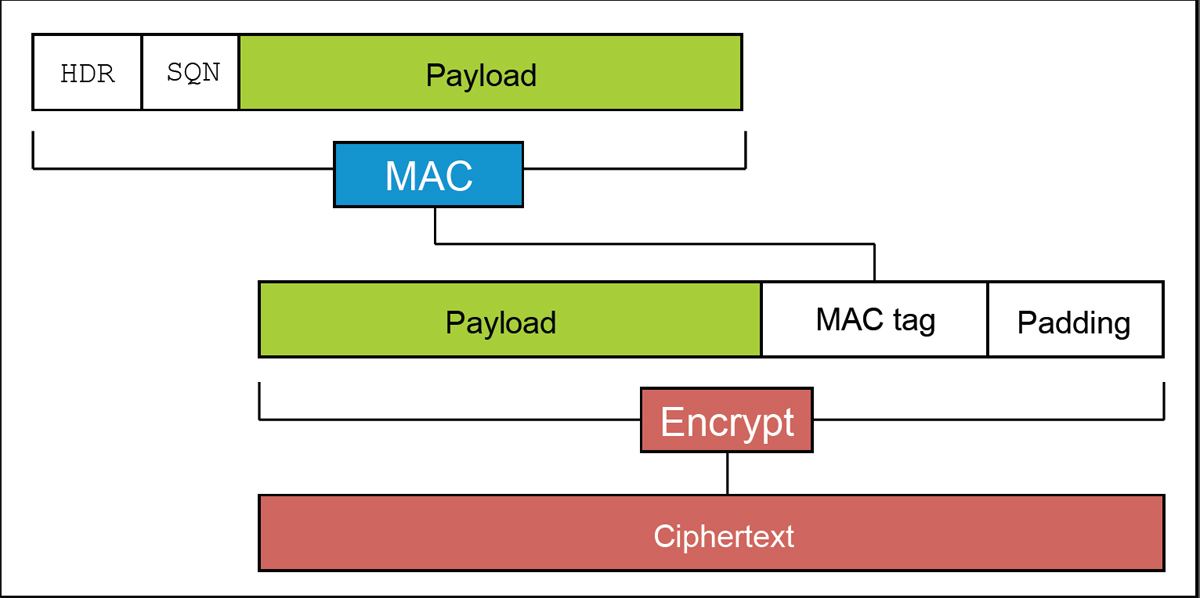
\includegraphics[width=0.5\textwidth]{tls-representation.jpg}
	\caption{Representation of TLS record.~\cite{alfardan2013lucky}}
	\label{fig:tls}
\end{figure}

\subsection{Accepting a record}
\label{sec:tls:accepting}
The RFC~\cite{ietf2008transport} does not describe the steps that need to be taken before accepting the payload of a received TLS record, fortunately the authors of the Lucky Thirteen attack have proposed a (incomplete) list of actions to be undertaken.
\begin{itemize}
  \item Check: is the ciphertext size a multiple of the block size?
  \item Check: is the ciphertext large enough to contain at least a zero-length record, a MAC tag of the required size and at least one byte of padding?
  \item Decrypt the ciphertext to recover the plaintext blocks: $P_i = D_k(C_i) \oplus C_{i-1}$.
  \item Is the padding of the appropriate format?
  \item Is the MAC correct (using the correct SEQ number and HDR field?
\end{itemize}



\section{Padding Oracle Attacks}
\label{sec:paddingoracle}

\subsection{}

\subsection{Bomb Oracles}
\label{sec:paddingoracle:bomb}




\section{Lucky Thirteen}
\label{sec:lucky}
The RFC of TLS 1.2~\cite{ietf2008transport} reports
\begin{quote}
Implementation note: Canvel et al. [CBCTIME] have demonstrated a timing attack on CBC padding based on the time required to compute the MAC.  In order to defend against this attack, implementations MUST ensure that record processing time is essentially the same whether or not the padding is correct.  In general, the best way to do this is to compute the MAC even if the padding is incorrect, and only then reject the packet.  For instance, if the pad appears to be incorrect, the implementation might assume a zero-length pad and then compute the MAC.  This leaves a small timing channel, since MAC performance depends to some extent on the size of the data fragment, but it is not believed to be large enough to be exploitable, due to the large block size of existing MACs and the small size of the timing signal.
\end{quote}

regular plaintext recovery of a block: 2\^23 connections
if base64 (cookies, http basic access authentication) used: 2\^23 -> 2\^19 connection per block
per cookie byte, using BEAST technique: 2\^13 connections



\section{The Future of TLS}
\label{sec:future}



\bibliographystyle{plainnat}
%\bibliographystyle{IEEEtran}
\bibliography{IEEEabrv,literature}
\end{document}






























